\section{Evaluation} \label{sec:evaluation}
The purpose of the evaluation is to establish knowledge concerning the possibility of creating a video game AI that matches the player's performance through the use of a genetic algorithm; as stated in the final problem statement.(See section XX)


\subsection{Method} \label{sec:eval_method}
the method of testing and evaluating said results will be constructed in the following manner.

Test subjects will be asked to play several games/levels of the product prototype whereof each game represent a new improved generation of our genetic algorithm. The general purpose is to account for the effectiveness of our genetic algorithm and the used method of alternations between the various states of the finite state machine, to evaluate whether our genetic algorithm is actually matching player performance.

There are several aspects that must be accounted for:

\begin{itemize}
\item How is player performance considered matched?
\item does our implementation of alternation between the various states of a finite state machine match player performance?
\end{itemize}


\textbf{Player Performance specification}


In section \ref{ssec:player-performance}, assessment of player performance is considered, and the following allegation of defining player performance matched, is specified as such;

The player performance will be considered matched if the attained score(points) of each game/generation of one single test participant is either equal or lower than the previous attained score(points acquired).

\textbf{Pre test specification}


A pre test of the prototype will be conducted to ensure that the implemented parameters of the prototype is optimal for testing to successfully answer to the final problem statement.
Additionally the pre test will determine the number of simulations and generations that will be used throughout a single test of one single test participant.

\newpage
\textbf{Main Test specification}

The test will consist of test participants playing levels of the prototype where each level is consisting of a new generation of the genetic algorithm.

The statistical test method and output data evaluation thereof will be conducted in accordance with the procedure listed by Field and Hole, 2003 \cite[pp. 265-277]{Field2003}, of how to design an experiment.

\begin{itemize}
\item Collected data: Scores

The data collected will consists of points(points collected throughout a single level played in the prototype) which can be categorized as ordinal data. This is due to the data being numerical where some ranking of the data values can be put into order.
\item Independent variable(s)

One independent variable will be modified, and is the alternation between the various states of the finite state machine in the prototype, as specified in the final problem statement.(See section XX)
\item experimental design

The experiment is considered of type experimental, as we look for differences between conditions which is the alternations of the independent variable.
\item repeated measures

Each participant will participate in each condition of the experiment and provide scores to each, and the design is therefore considered a repeated measure design.
\item Non Parametric data

The data is considered non-parametric as the collected data is of type ordinal data.

\end{itemize}

%!TEX root = ../../main.tex
\subsection{Pre Test} \label{ssec:pretest}
This chapter describes the pre-test that is mentioned above.
The chapter will describe the acquisition of data the evaluation of the gathered results.

\subsubsection{Purpose}
The purpose of this pre-test is to test the implementation and test its eligibility for the main testing.
The pre-test will produce observations for use in further development of the implementation and for use in the discussion and re-design.
Because the main test will be conducted on people outside of a lab environment, we want reduce the time required by the test participants.
The ultimate purpose of the pre-test is to establish how many generations are needed for the final test.

\subsubsection{Method}
The pre-test will be conducted with ourselves as subjects and will not require any outside test participants.

The test conductor will run 20 generations of the game and note any observations regarding troubleshooting, initial failures, and missing functionalities.
The data required from the games logs are the genes for the ghosts, the time taken to do a play-through of the game followed by the 10 simulations.
The time will be taken manually by the test conductor.

The observations considered most critical to the conduction of the main test will be attended to during the test and the test will be restarted.

The test will be done under the assumption that as the generations will progress, the alterations on the genes of the ghosts, done by the GA, will start to stabilize.
The point where the genes start to stabilize will be the point where we main test can be terminated.

To find this point the content of the genes are required the average value of the genes per generation, per ghost, per mode.
When the average values will be similar to the previous value over a range of generations, the genes can be considered to be stabilizing.

\subsubsection{Procedure}
\begin{enumerate}
	\item Gather sample and record time.
	\begin{enumerate}
		\item Play game (F1)
		\item Run simulation (F5)
	\end{enumerate}
	\item Note observations and errors.
	\item Copy simulation data (F8)
	\item Gather sample and record time.
	\begin{enumerate}
		\item Play improved game (F9)
		\item Run simulations (F5)
	\end{enumerate}
	\item Note observations and errors
	\item Copy simulation data (F8)
	\item Repeat from step 4
\end{enumerate}

\subsubsection{Results}
The gathered list of observations is listed below.

\subsubsection*{Comments}

\begin{itemize}
	\item Ghosts go together (ghosts have the same movements, making them walk on top of each other)
	\item Ghosts appear to be inactive for too long after power pellet.
	\item When the player dies and the simulations are running, the player continues down the predetermined path until it hits a wall, upon death.
	\item When the player dies during a run, then for the following simulations, upon the time of death of the player, the pac-man becomes idle and is not moving until death occurs.
	\item Ghosts appear to stop moving for a considerable amount of time during simulations.
	\item The blue ghost appear to seek the upper left corner to circulate in several simulations following a somewhat similar pattern.
	\item Some ghosts perform similar movement in several simulations.
	\item When consumed, ghosts spawn instantly on the spawn point, Resulting in instant death if ghost is consumed on this area, resulting in spawning almost simultaneously on the same location.
	\item When ghosts are consumed, they spawn and occasionally don’t move for several seconds from the spawning location.
	\item In simulations where the player died, and therefore is standing still on the location of death, the ghosts seem to move to the upper left corner, where they circulate.
	\item One ghost(orange) didn’t move for almost an entire simulation.
	\item The ghosts loose all sense of “intelligence” when pac-man is standing still and they face the wall.
\end{itemize}

\subsubsection*{Timing}
The table below consists of the time it took to do a player recording together with the following ten simulations and copying the results from that generations test results into a separate document.
\begin{table}[!htbp]
\centering
\begin{tabular}{l c}
generations & Time recorded \\
\hline
1 & 3:15 \\
2 & 2:00 \\
3 & 2:51 \\
4 & 2:47 \\
5 & 1:37 \\
6 & 2:18 \\
7 & 3:19 \\
8 & 2:19 \\
9 & 2:06 \\
10 & 2:55 \\
11 & 4:01 \\
12 & 1:56 \\
13 & 3:33 \\
14 & 2:59 \\
15 & 1:44 \\
16 & 3:22 \\
17 & 2:35 \\
18 & 3:00 \\
19 & 2:21 \\
20 & 3:23 \\
\hline
\end{tabular}
\caption{Times per generation during pre-test}\label{tab:times}
\end{table}

The total time was 54.12

The average play-through took 2.43 minutes.


\subsubsection*{Genes}
The collected gene-data from the logs can be found on the digital appendix.
Below will be the processed data.

\begin{figure}[!htbp]
	\centering
	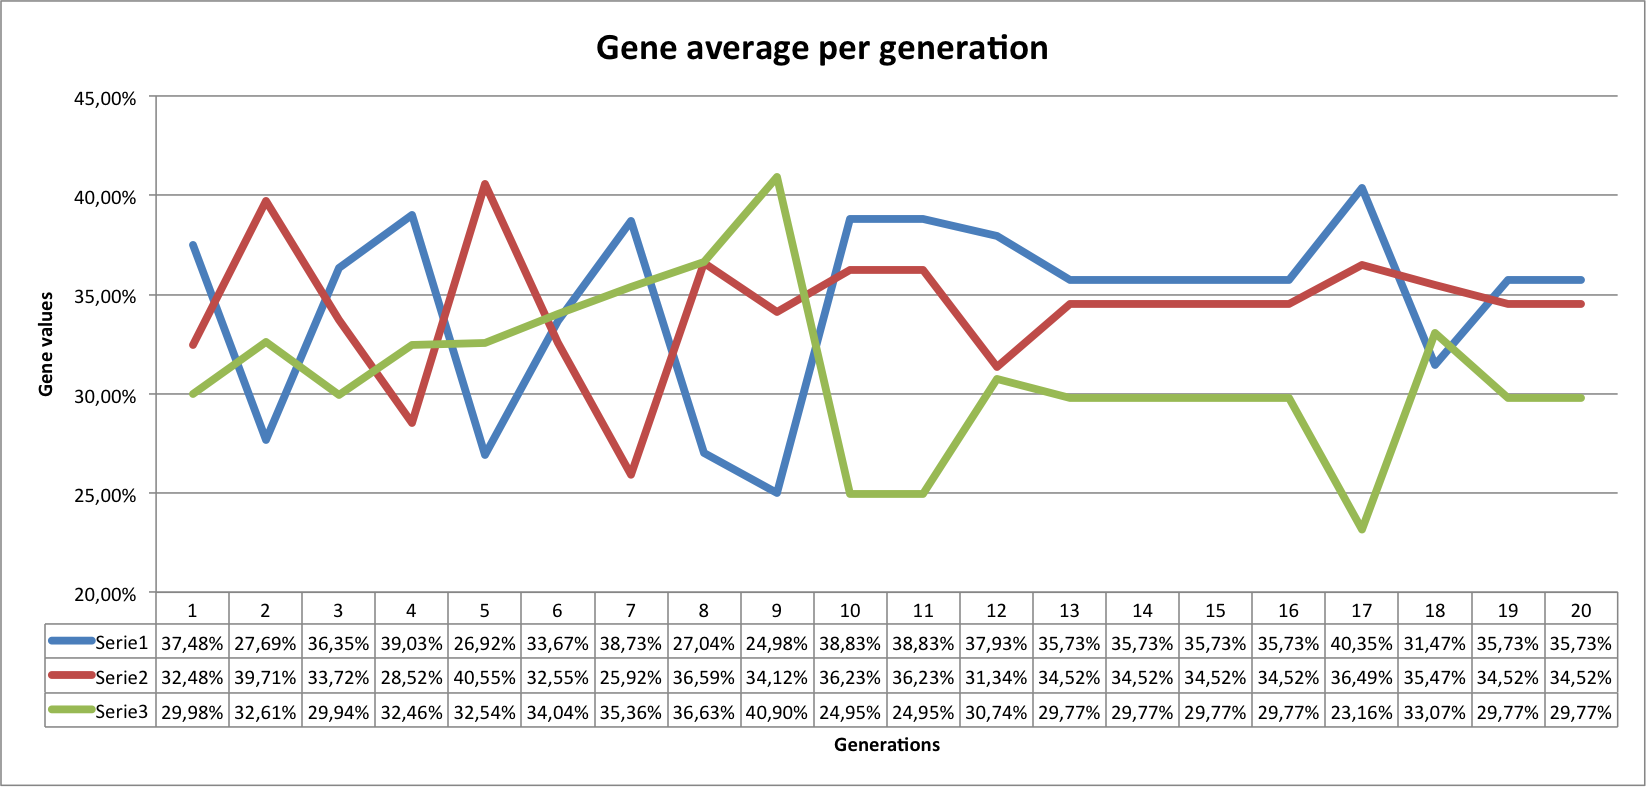
\includegraphics[width=0.85\textwidth]{pretest_average.png}
	\caption{Averages of genes over generations.}
	\label{fig:pretest_average}
\end{figure}

\begin{figure}[!htbp]
	\centering
	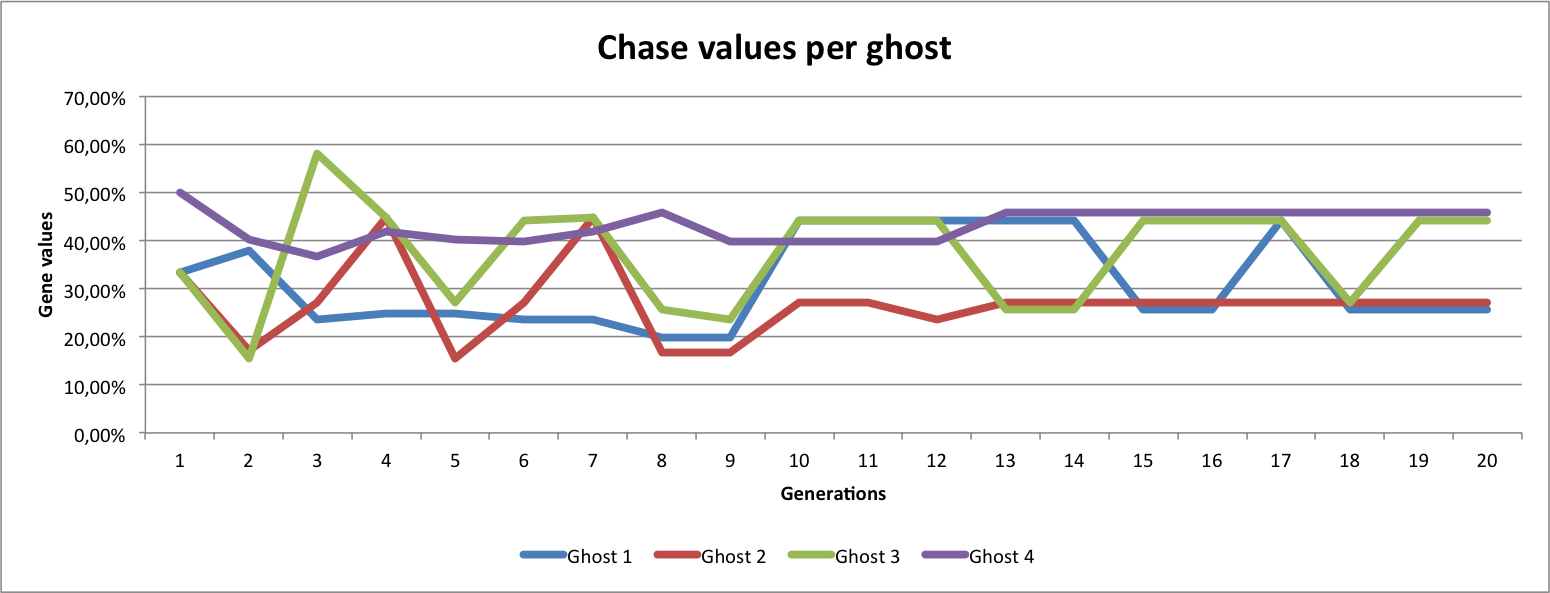
\includegraphics[width=0.75\textwidth]{pretest_chase.png}
	\caption{The recorded chase mode values over generations.}
	\label{fig:pretest_chase}
\end{figure}

\begin{figure}[!htbp]
	\centering
	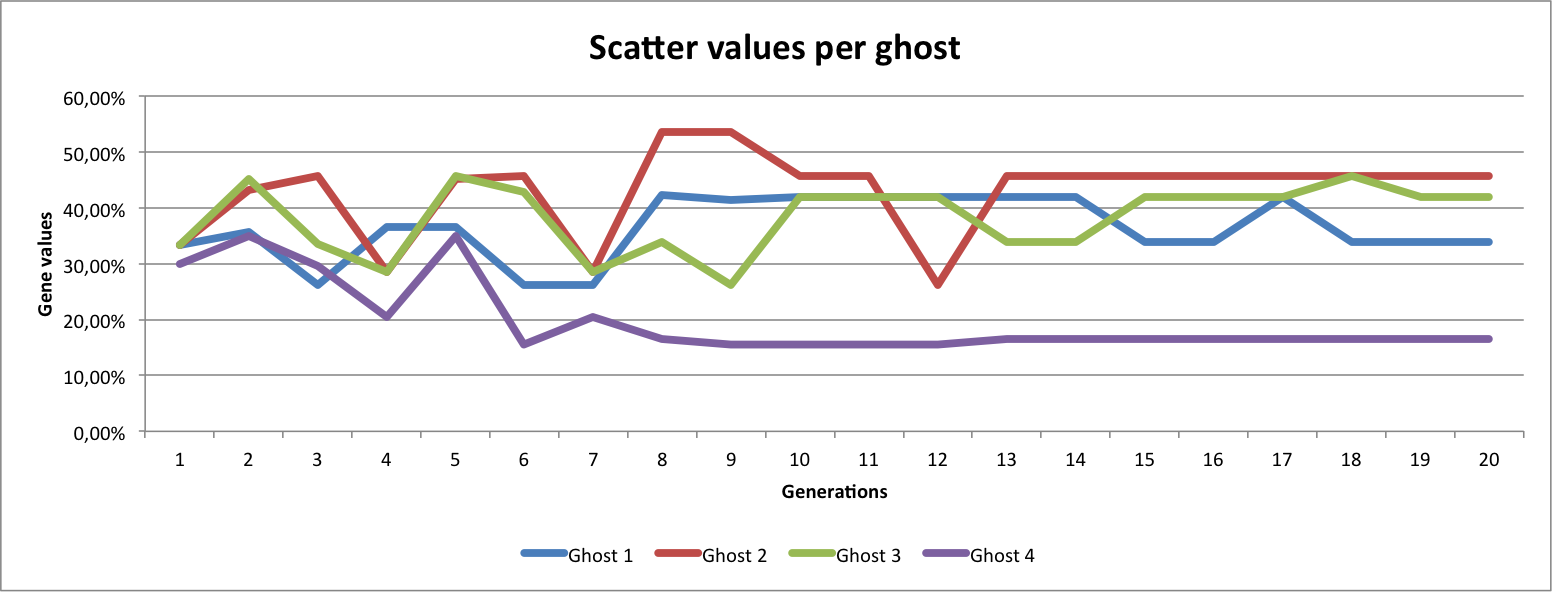
\includegraphics[width=0.75\textwidth]{pretest_scatter.png}
	\caption{The recorded scatter mode values over generations.}
	\label{fig:pretest_scatter}
\end{figure}

\begin{figure}[!htbp]
	\centering
	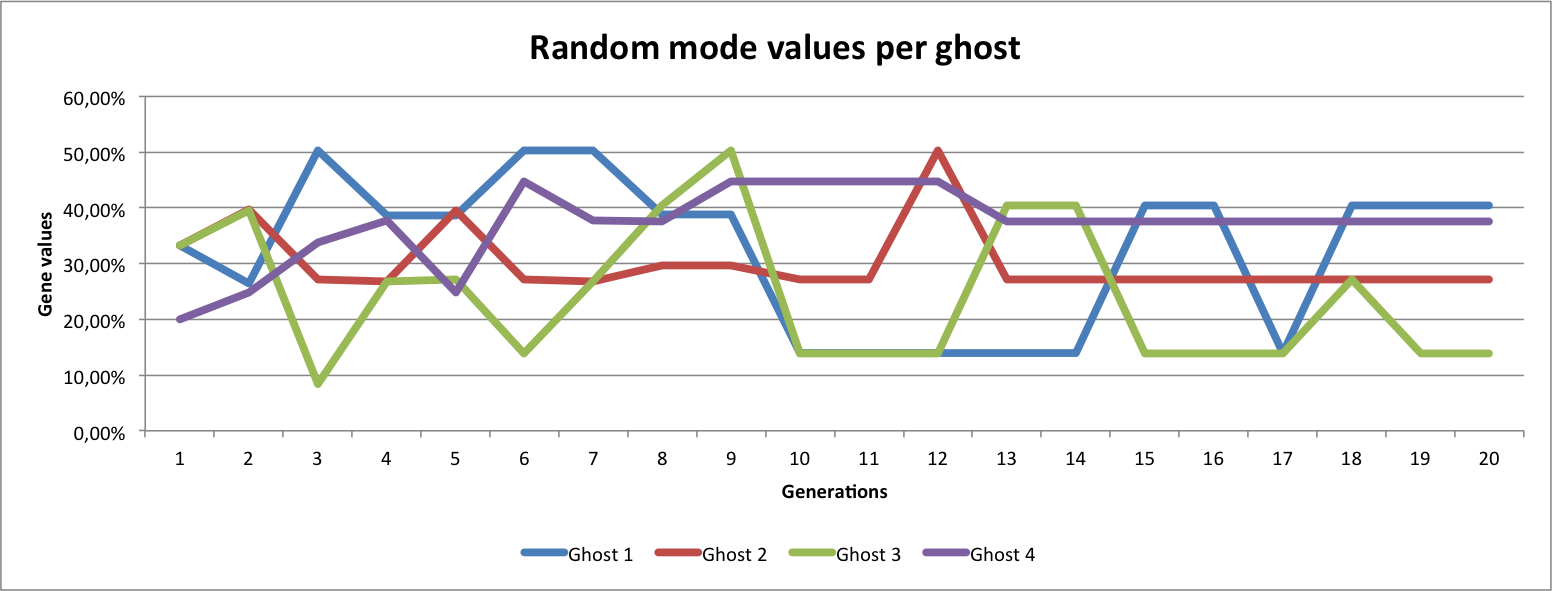
\includegraphics[width=0.75\textwidth]{pretest_random.png}
	\caption{The recorded random mode values over generations.}
	\label{fig:pretest_random}
\end{figure}

\subsubsection{Result Evaluation}
Of the comments shown above, the observation that the ghost spend too long in flee mode was fixed during the testing as it greatly reduced the time the ghosts were active during a game, which can be considered a bias.
The new time the ghosts spend in flee mode is reduced to two and a half seconds.

The ghosts would all gather in the same corner during scatter mode.
This is not intentional and was fixed during testing.
The ghosts now go to a separate corner of the maze during scatter mode.

\subsubsection*{Genes}
By analyzing the genes we want to find the point where the genes start to stabilize and the variations in the genes do not vary.
This point is considered where the GA can no longer make alterations that can match the player performance any better than what it already has.
At this point we speculate that the values of the genes will not be altered any further.
The user test should be terminated at this point.

Figure~\ref{fig:pretest_average} shows average values of the genes for each mode for each ghost in each generation.
If the average is the same as the previous value it means that the sum of the genes values for each ghost in that generation has not changed in the new generation.
This could mean that the genes are unchanged or swapped within the same generation.

It can be seen on figure~\ref{fig:pretest_average} that the genes start to stabilize shortly after the tenth generation with only a few spikes in the averages.

In figures~\ref{fig:pretest_chase},~\ref{fig:pretest_scatter}, and~\ref{fig:pretest_random} the values of a specific mode within the genes are placed up against their generations.
These also indicate that the genes start to stabilize around the tenth generation with only few variations within the range of the lowest and highest values.

\subsubsection*{Time}
Because we will be conducting the test on random sampled participants without appointment we want to minimize the amount of time needed by the participant.
We see 30 minutes as being an acceptable timeframe to ask of people for the test.

It is seen in the results that a test with 20 generations will take around 54 minutes, which means that we can do 11 generations within 30 minutes.
Together with the results from the gene comparison above, which suggests that the genes will stabilize around generation 10, we estimate that 10 generations will be adequate for the each test participant.

\subsection{Procedure}
Taylor-Powell1998
\subsubsection{Questionnaire}
There is a possibility of collecting biased data if the test subjects perform on the same skill level.
If the test subjects happen to be at the same skill level, we would not be able to determinate if our GA is working properly, making them equally good, or if they are equal in skill. To avoid this bias we wish to collect quantitative data in relation to how much our population differs from each other based on the test subject's opinion of their own abilities in games.

The quantitative information will be collected through a questionnaire that has been designed after the guidelines by Ellen Powell's  \cite{Taylor-Powell1998} Taking these guidelines into consideration we have designed 5 questions that will ask the test subject to reflect on experience as well as place them on a likert scale before conducting the test. The purpose of the 5 questions will be described, but not stated in this report as they can be found in the appendix (XX).

Question 1 is a general question that is designed to get the test subjects overall ability in games. We would like to know if we are dealing with experienced gamers who understand a games interaction and can defeat an expected difficulty. According to Powell's guidelines, a negative response option should always be provided, in case the subject is inexperienced in games and do not play games at all. Because of this, we have the option "Never" the test subjects can answer, or if they feel they have more expertise, can they answer between "Sometime", "Often" and "More often".

Question 2 asks the test subject to rate their current gaming skill, this gives us an idea of what level the test subject prefer playing. In the previous question, the test subject may have answered "Sometimes" however performs exceptionally in games with which we can consider them good at defeating a games difficulty.

As described earlier in section (XX) our game is not a copy of the original Pac-man, however there is similarities with the classic arcade game and we will therefore refer the following questions to this specific game in order to help us explain our GA for the test subjects.

Question 3 will be considered a control question. We cannot expect all test subjects knowing what Pac-Man is, and will therefore have to ensure us they have a descent knowledge of the game. The gameplay will be explained no matter what, but if answering no, will the test observes go more into details about the gameplay. If answering yes will the test participant have to answering question 4 as well.

Question 4 is designed to recall their own memory. The test subjects may be familiar with Pac-Man but have they only heard of it, or have they actually played before? In that case would we like to know if they remember Pac-Man's original difficulty. We will assume the test subjects have a good knowledge of Pac-Man if giving a positive response, and a poor knowledge of Pac-Man if giving a negative response. In Question 5 can they compare themselves to Pac-Man's difficulty and place themselves on a likert-scale.

Question 5 will be visualized into a graph that illustrates the distribution.

These questions have been designed to help us illustrate a distribution of the skill level according to the test subjects. For this matter are we not looking into finding a relationship between the responses and will not conduct a chi-square test on the non-parametric data.

\subsubsection{Testing}
Testing found place on several location and was conducted on 21 participants in an estimated time of 30 minutes each.
It makes use of a convenience sampling that does not prefer a specific population, but test on volunteering participant that are readily available. \cite{Exploarable2009} In our FPS is there no current population required, and we make therefore use of this sampling method. The testing happened December 2014, in the following locations:
\begin{itemize}
\item 15 of the test found place in the test participant?s home
\item 1 in a library
\item 5 at AAU University
 \end{itemize}

\subsubsection{Test Design}
The performed test is considered an experimental design test that uses repeated measures.
Repeated measures are collecting data from the same test participants and compare several conditions to each other trying to observe a plausible effect. \cite{Shuttleworth2009} In our case are participant contributing data 10 times each time they play an improved generation.

We are receiving reliable data because the repeated measure requires same participants, that are an advantage for us, however can there still be some disadvantages we need to consider. According to Shuttleworth, 2009 are there biased effects that can have bad influence on the data. These effects are known as carryover, practice and conversely. \cite{Shuttleworth2009}

\begin{itemize}
\item Carryover effect
The test participants? first condition is still fresh in mind or body and can affect the second condition.

\item Practice effect
The test participant can improve over time and become better for each task.

\item Conversely effect
The test participants become bored which could influence their performance in a negative way. In addition ending the gameplay without completing all 10 generations, resulting in small sample without statistical significance.

 \end{itemize}


\subsubsection{Test Setup}
The test does not require any specific location it was however recommended the test subject was comfortable for the 30 minutes. For each test was 1 test observer present and tasked to stay nearby in order to fulfill some of the procedures as described in Test execution.

The test material needed for testing, includes:
\begin{itemize}
\item	Portable computer (PC)
\item	Game prototype
\item	Questionnaire
 \end{itemize}

Test execution
Each test scenario should follow a formulated test structure that ensures every test data is gathered identical. It would be a potential bias if several data have been measured through separate methods, and conducted differently making it inconsistent. It is the test observer's responsibility to follow this structure and save each measured data set in a single document, along with the answers from the questionnaire.
The following contexts will give a detailed explanation of the test structure point for point.

Inform the test participant the testing will take approximately 30 minutes, and are expected to play 10 rounds of the prototype. Ensure the test participants know the gameplay and rules, and give them space each time they play.

\begin{enumerate}
\item	Open a new empty test document (Player document)
A test observer opens a new empty document and write the numbers 1, 2, 3, 4, 5 corresponding to the 5 questions in the questionnaire.

\item Introduce questionnaire
Test observers give an introduction to the questionnaire and write down the test subjects answers in front of the following number to the question in the document.
End the questionnaire with a dashed line, press enter and write, ?test start? under the dashed line.

\item Play game (F1)
Two play modes are available; F2 is for two-players but inactive, therefore press F1 for single player and to start the game.

\item Run simulation (F5)
When the single play-through has ended, press F5 to run 10 automatics simulations of played game. Make sure the test participant does not observe any actions occurring on the screen whilst it takes place.

\item Paste data (simulations) (F8)
Stay in the game and press F8 to copy simulation data, open the test.txt document were the simulation data have been stored, copy all text, paste into player document, press enter and add a new dashed line, press enter again.

\item Play improved game (F9)
Press F9 to play improved game.

\item Run simulations (F5)
When the single play-through has ended, press F5 to run 10 automatics simulations of played game. Make sure the test participant does not observe any actions occurring on the screen whilst it takes place.

\item Paste data into document (F8)
Stay in the game and press F8 to copy simulation data, open the test.txt document were the simulation data have been stored, copy all text, paste into player document, press enter and add a new dashed line, press enter again.

\item Repeat point 6, 7, 8 (10 times)

\item If a crash occurs, describe data.
If pressed any other buttons as mentioned above can a crash occurs. If this happens are the measured data considered useless and test subject has to start the test all over.
 \end{enumerate}

End the testing by informing the test participant the game is terminated.



\newpage
\subsection{Test Data and Results}
The following content is the combined data collected from the conducted test accompanied by a description thereof. discussion and interpretation of the content will be conducted in evaluation discussion(See section \ref{resulteval}).

\subsubsection{Main test data}
The acquired main test data consist of the following content(See figure \ref{fig:testdata} for data snippet).

The entire list of recorded data can be accessed in the digital appendix.(See appendix XX)

\begin{figure}[!htbp]
\centering
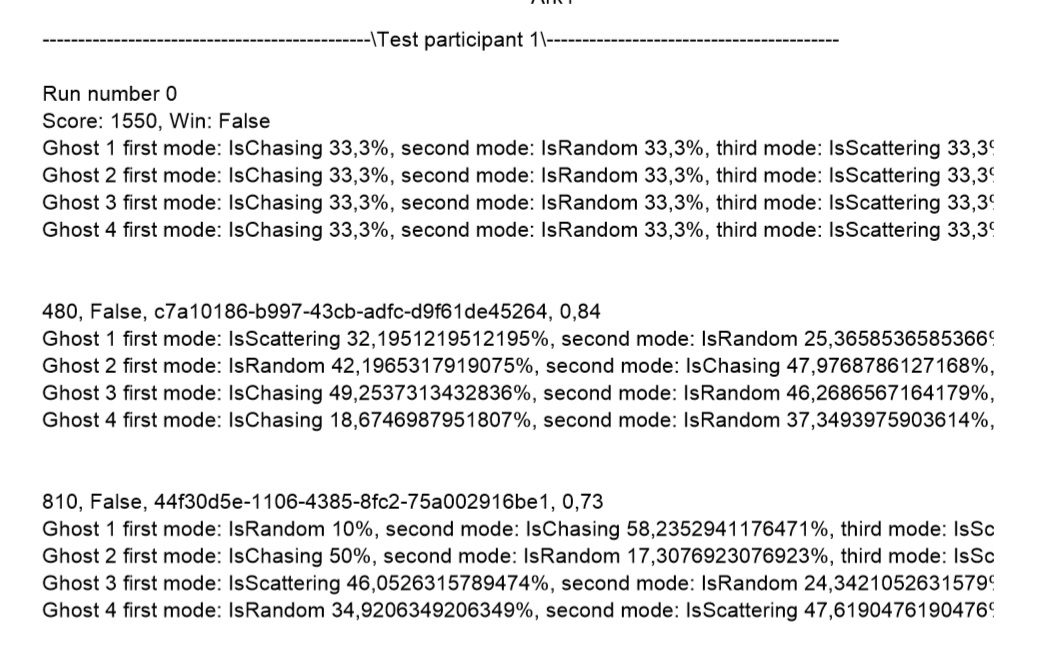
\includegraphics[scale=0.5]{testdata.jpg}
\caption{test data representation}
\label{fig:testdata}
\end{figure}


\newpage

The collected data consists of the following elements in descending order:

\begin{itemize}
\item  \textbf{Text participant}

Represent the participant number running from 1-21.
\item  \textbf{Run number}

Represent the current generation that the test participant is currently playing. Ranges from 0-9.
\item  \textbf{Score}

Represent the amount of points attained in the current generation/level.
\item  \textbf{Win}

Represent whether or not the test participant won the generation/level in a boolean statement. Win:True is the player won and Win:False is the player lost.
\item  \textbf{Ghost Mode}

Ghost 1-4 mode represent each of the four ghosts.


IsChasing, isRandom and isScattering represent the ghost Modes.(See section XX for mode description)

The percentages represent the length that each mode is active.

the order(sequence of modes) of each ghosts represent the order that the MonsterModes are switched between.(See section XX for documentation) Changing the order of the modes will change the time they are active during play or simulation in the prototype.
\end{itemize}

\newpage
Figure \ref{fig:testdata_simulation} depicts the data acquired of the simulations. After each level/generation played by a test participant there are 10 simulations.
The data recorded consists of the following elements for each simulation:

\begin{figure}[!htbp]
\centering
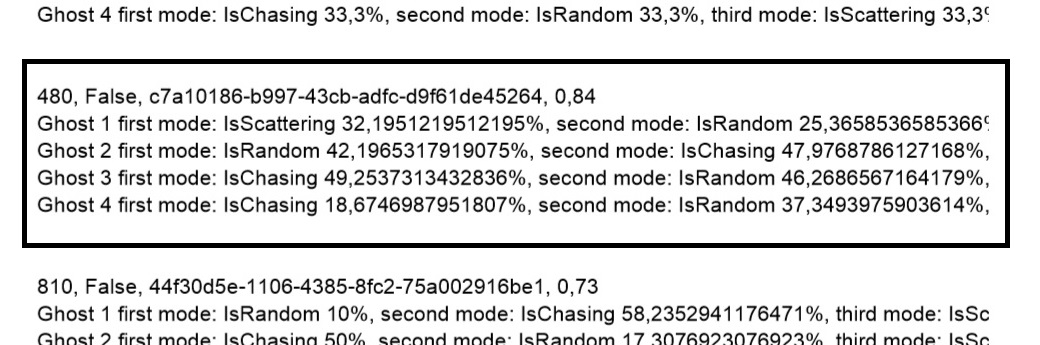
\includegraphics[scale=0.5]{testdata_simulation.jpg}
\caption{test data representation: Simulation}
\label{fig:testdata_simulation}
\end{figure}

\begin{itemize}
\item \textbf{first occurring number}

Represents the points collected during the entire simulation.

\item  \textbf{false/true}

Similar to the played level/generation, the boolean describes if the level is won or lost.

\item \textbf{<listCycles>}

The list represents the genes within each chromosome which are the solution to the given simulation.

\item \textbf{Fitness score}

The number ranging from 0-1 is the assigned fitness score to the current simulation. Depicted as 0.84 in the snippet(See figure \ref{fig:testdata_simulation})
\end{itemize}
\newpage
\subsubsection{Player level/generation points}
The following snippet(See figure \ref{fig:point_collection}) depicts the points collected by each one of the test participants from each generation/level.


The rows is the points collected from all test participants for each generation/level.

The columns are points collected by each test participant over the course of playing against the improved genetic algorithm over 10 generations. Ranging from generation 0 to generation 9(GEN 0 - GEN 9).
\begin{figure}[!htbp]
\centering
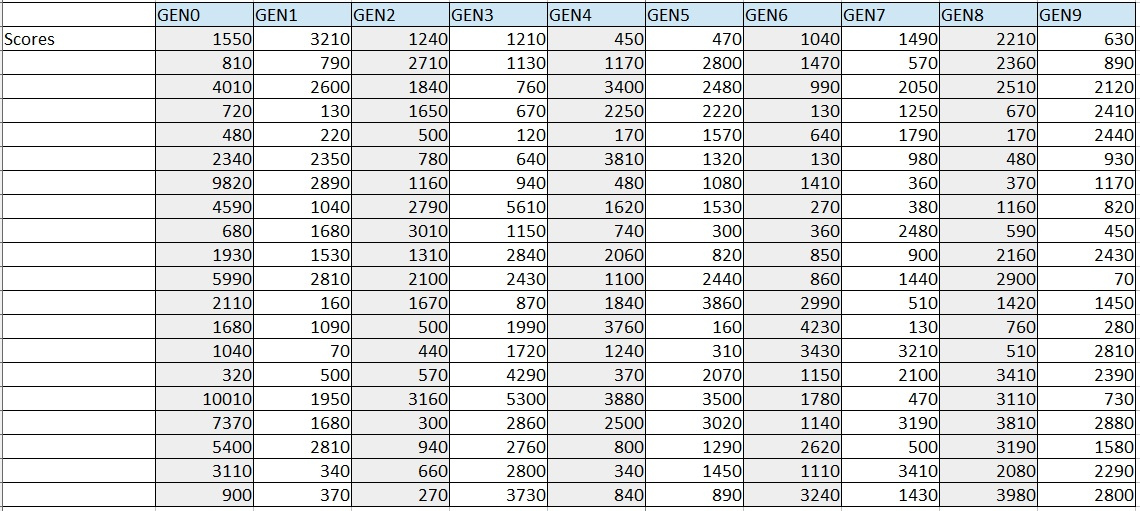
\includegraphics[scale=0.5]{player_points.jpg}
\caption{point collection}
\label{fig:point_collection}
\end{figure}

\newpage
\subsubsection{Questionnaire data}
The following data are the responses from the questionnaire acquired from the test participants.

\begin{itemize}
\item \textbf{How often do you play computer games?}
\begin{itemize}
\item 2 participants answered: never.
\item 6 test participants answered: Sometimes.
\item 5 test participants answered: Often.
\item 8 test participants answered: Very often.
\end{itemize}
\item \textbf{Please rate your skill in general computer/console games(scale from 1-10}

Figure \ref{fig:question2} represent the answer distribution on a scale from 1-10.

\begin{figure}[!htbp]
\centering
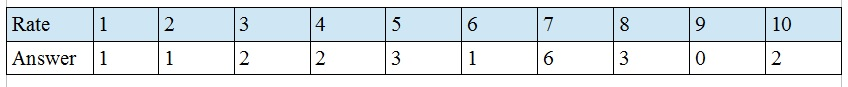
\includegraphics[scale=0.5]{question2.jpg}
\caption{test participant assessment of computer/console playing skill}
\label{fig:question2}
\end{figure}

\item \textbf{Are you familiar with the classic arcade game Pac-man}
\begin{itemize}
\item 21 test participants answered: Yes.
\item 0 test participants answered: No.
\end{itemize}
\item \textbf{If answering yes to the previous question, how often did/do you play it?}
\begin{itemize}
\item 5 test participants answered: Never.
\item 13 test participants answered: Sometimes.
\item 3 test participants answered: Often.
\item 0 test participants answered: Very often.
\end{itemize}
\item \textbf{Please rate your current skill level in the classic arcade game Pac-man(scale from 1-10)}

\begin{figure}[!htbp]
\centering
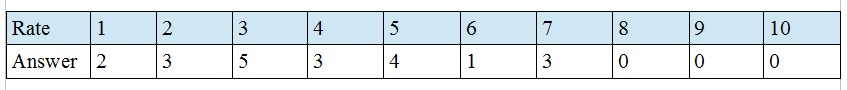
\includegraphics[scale=0.5]{question5.jpg}
\caption{test participant assessment of Pac-man playing skill}
\label{fig:question5}
\end{figure}

Figure \ref{fig:question5} represent the answer distribution on a scale from 1-10.
\end{itemize}


\newpage
\subsection{Result evaluation} \label{resulteval}

As specified in the method section(See section \ref{sec:eval_method}) we state that the independent variable is the alternation between the various states of the finite state machine.

The dependant variable is amount of points attained in each generation/level, whereof each condition is repeated by the same test participant.

also specified is the player performance which is  considered matched if the attained score(points) of each game/generation of one single test participant is either equal or lower than the previous attained score(points acquired).

In order to discuss whether or not the attained score is equal or less than the previous attained score(points acquired) we can construct a visualisation of the collected output data which is the points attained by the test participants in our repeated measured test design.
As the data type is non-parametric, a boxplot can be used to visualise the distribution.

\begin{figure}[h!]
\centering
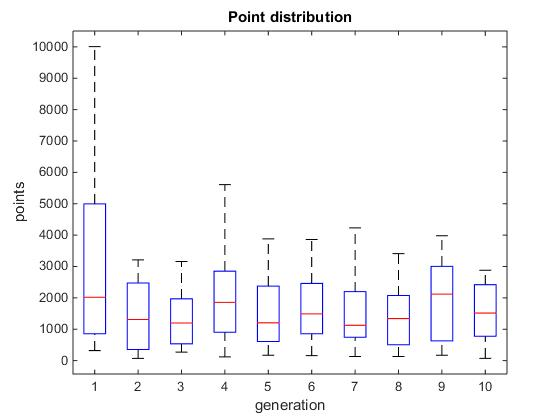
\includegraphics[scale=0.6]{point_boxplot.jpg}
\caption{point distribution boxplot}
\label{fig:boxplot_points}
\end{figure}

\subsubsection{point data distribution: Boxplot visualisation}

The boxplot seen on figure \ref{fig:boxplot_points} visualise the distribution of points for each generation, and makes it possible to account for the variance.

From the visualisation of point distribution the following can be observed:

The median, as the value representing the separation of the higher and lower half of the data distribution, shows a different median value in each of the generations. It can be observed that the median increases 4 times and decreases 5 times, but within a range of values somewhat ranging from 1000 points to 2100 points approximately.

The outliners represent the range of points attained in each generation and specify the highest and smallest amount of points collected within each generation from all the test participants in one single generation.

The first generation outliner shows the highest attained score of approximately 10000 points and the lowest being somewhat close to 3-400 points. The bottom outliner is observably very similar in each generation. From generation 2-10 a noticeable  decrease in the range of points collected in the following generations occur, much unlike generation 1.

The distribution of data is also indicated by the observed quartiles and range of them. The quartiles indicates that 50 percent of the data lies within the quartiles. Observably is the quartile range. From generation 2-10 the range of values both for the outliners but also the quartiles, illustrates that the data distribution is much smaller compared to the first generation. Between generation 2-10 there is a much smaller diversity in the range of both outliners and quartiles.

Lastly the skewness of the median compared to the placement within each quartile indicates that 25 percent of the test participant is within a smaller range of distribution compared to the 25 percent above the median, which has a wider range of distribution. Thus a larger amount of test participants(25 percent) attained a somewhat similar score below the median, compared to the distribution above the median.

\subsubsection{Delta score data distribution: box plot visualisation}

in addition to the visualisation of point distribution over 10 generations, we can also assess the amount of difference between the points collected in each generation. This will make it possible to observe if there is some difference in the points collected over each of the generations, but also specify how much difference of points collected there is over each generation. Thus it will be possible to evaluate whether or not the points collected is equal, increased or lowered compared to the previous attained scores over 10 generations and how much.

The delta score is calculated by conducting the following calculations:

[Generation 1 points] -[generation 2 points]

[generation 2 points] - [generation 3 points]...[]

The delta score is calculated both for absolute values, meaning that we only look for the positive amount of difference, and for accurate values, meaning that also negative values are specified.

Thus it will be possible to observe the amount of difference in points obtained over the generations, but also whether or not the difference is positive or negative.

Figure \ref{fig:deltascore_positive} illustrates the positive deltascores of the amount of difference between the points acquired for each of the test participants over each of the 10 generations.

\begin{figure}[h!]
\centering
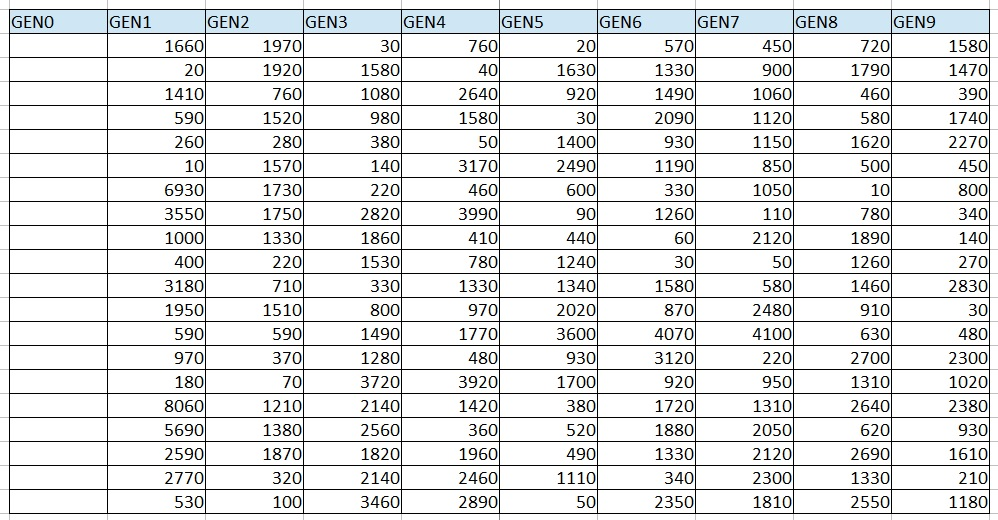
\includegraphics[scale=0.6]{deltascore_positive.jpg}
\caption{deltascores with positive amounts}
\label{fig:deltascore_positive}
\end{figure}


Figure \ref{fig:deltascore_negative} illustrates the positive and negative deltascores of the amount of difference between the points acquired for each of the test participants over each of the 10 generations. Thus also indicating the amount of difference is either positive or negative.

The following boxplots figures illustrates the amount of variance of the points collected. Figure \ref{fig:delta_positive} illustrates the distribution of postive amounts of variance. Figure \ref{fig:delta_negative} illustrates the distribution of both positive and negative amounts of variance.

\begin{figure}[h!]
\centering
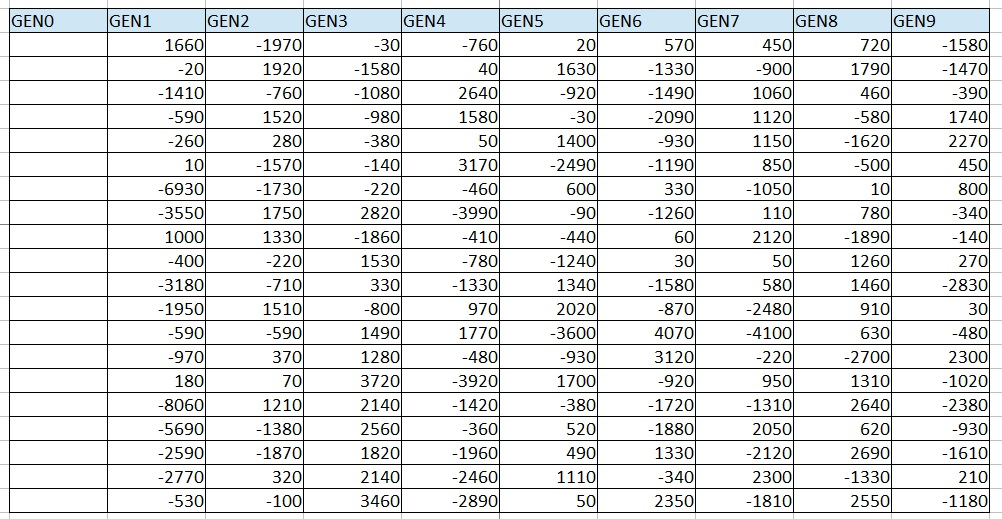
\includegraphics[scale=0.6]{deltascore_negative.jpg}
\caption{deltascores with positive and negative amounts: Boxplot}
\label{fig:deltascore_negative}
\end{figure}






\begin{figure}[h!]
\centering
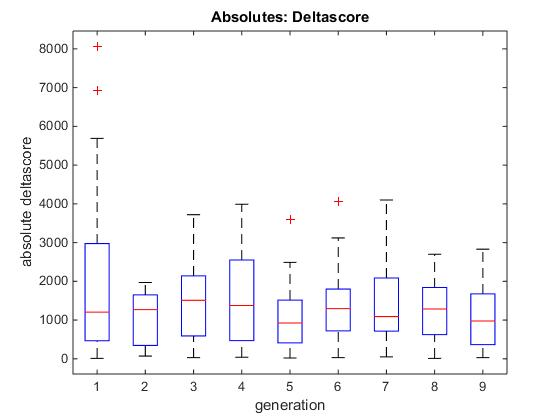
\includegraphics[scale=0.6]{deltascore_absolutes_boxplot.jpg}
\caption{Deltascores with positive amounts}
\label{fig:delta_positive}
\end{figure}


\begin{figure}[h!]
\centering
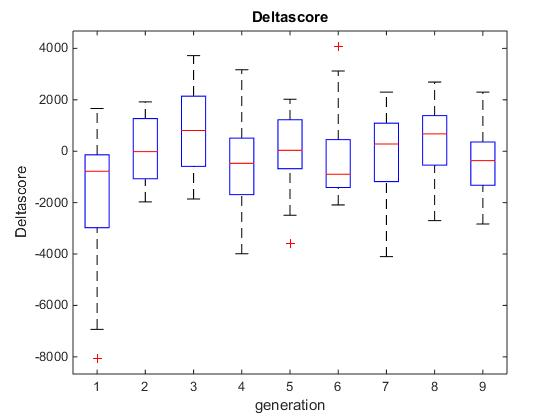
\includegraphics[scale=0.6]{deltascore_includeNegative_boxplot.jpg}
\caption{Deltascores with positive and negative amounts: Boxplot}
\label{fig:delta_negative}
\end{figure}

Boxplot figure \ref{fig:delta_positive} illustrates that there is an large change in the points attained from generation 1 to generation 2 as indicated by the outliners in generation 1. Thus it means that a player had a score, either low or high in generation 1, and increased or decreased the score by 8000 points in the next generation.

From generation 2 to generation 9, the quartiles and medians show that the amount of variance in points is occurring. The quartiles show that the distribution of 50  percent of the points attained is ranging from approximately 300-2000 points. Additionally with the boxplot, it can be observed that a skewing of the median in the quartiles of ex. generation 7 that 25 percent of the distribution, in the amount of variance, is somewhat between 600-1000.

In figure \ref{fig:delta_negative} we can observe similar data as in figure \ref{fig:delta_positive}, but with the specified negative or positive amount of variance. Thus it is observable that the distribution of variance is not only negative, but also positive. A positive amount of variance can be observed 5 times, and a negative amount of variance is observed 3 times over the generations.

\newpage
\subsection{Evaluation discussion}
The following content is a discussion of the evaluated results and thus it will be deducted whether or not the data will help us to answer to the final problem statement. And if the final problem statement has been successfully answered.

As described in the method chapter, See section \ref{sec:eval_method}, we define matched player performance in the following manner:

The player performance will be considered matched if the attained score(points) of each game/generation of one single test participant is either equal or lower than the previous attained score(points acquired).

In the evaluation of data, we find that the deltascore, through the visualisation of a boxplot, that the amount of variance in points is increasing and decreasing.

To successfully state that player performance is matched, the deltascore should be either 0, indicating that there is no change in the points attained by the test participant over the generations, or that the amount of variance should be increased, but be observed in figure boxplot \ref{fig:delta_negative} as negative, indicating that the player score over the generations is continuously decreasing with some amount.

Thus the point boxplot(See figure \ref{fig:boxplot_points}) show a varied distribution of points collected by the test participants and the deltascores show the amount of variance of points attained over the generations which is observed as both positive and negative amounts.

The discussion of how player performance criteria and definitions has been met and conducted and what the general test results implies in terms of the final problem statement will be discussed in the following discussion chapter.

